%setwd("S:\\synthpop 14112017") 
%## Produce .tex file from .Rnw file
%Sweave("inference.Rnw")
%## Produce .pdf file from .tex file
%tools::texi2pdf("inference.tex")



\documentclass[12pt]{article}

\usepackage{amssymb,amsmath,latexsym,graphics,authblk,url,setspace,caption}


%\usepackage[pdftex]{graphicx}
\usepackage{epstopdf} 
\usepackage{enumerate}
\usepackage{float}
\usepackage{color}
\usepackage{amssymb}

\usepackage{setspace}
\usepackage{amsmath}
\usepackage{hyperref}
\usepackage{verbatim}
\usepackage{algorithm}
\usepackage{algpseudocode}
\usepackage{color}
\usepackage{footnote}
\usepackage{threeparttable}
\usepackage{caption}
\usepackage{setspace}



%\usepackage{breqn}

\usepackage[square,sort,comma,numbers]{natbib}

\usepackage[portrait, margin=0.8in]{geometry}

\title{Practical privacy metrics for synthetic data}
\author{Gillian M Raab,  Beata Nowok \& Chris Dibben}


\renewcommand{\baselinestretch}{1.5} % 1.5 denotes double spacing. Changing it will change the spacing

% \VignetteIndexEntry{Disclosure}

\usepackage{Sweave}
\begin{document}
\Sconcordance{concordance:disclosure.tex:disclosure.Rnw:1 40 1 1 0 2 1 1 4 44 1 1 %
2 1 0 1 2 1 0 1 1 1 2 1 0 1 1 11 0 1 2 37 1 1 2 1 0 1 2 1 0 1 1 16 0 %
1 2 15 1 1 2 15 0 1 2 10 1 1 4 31 0 1 2 21 1 1 3 2 0 1 1 18 0 1 2 9 %
1 1 3 2 0 1 1 14 0 1 2 223 1 1 2 17 0 1 2 3 1}



\maketitle
\begin{abstract}
From version 1.8-1 the \texttt{synthpop} package includes functions to calculate identity and attribute disclosure risk measures for the original records using information obtained from the corresponding synthetic data. The basic function \texttt{disclosure} calculates identity disclosure for a set of quasi-identifiers (keys) and attribute disclosure for one variable specified as a target from the same set of keys. The second function \texttt{disclosure.summary} is a wrapper for the first and it presents summary results for a set of targets in the data set. This short paper explains the measures of disclosure risk and documents how they are calculated. We recommend two measures: $RepU$ (replicated uniques) for identity
disclosure and $DiSCO$ (disclosive in synthetic and correct in the original) for attribute disclosure. Both
are expressed a \% of the original records and both can be compared to similar measures calculated from the original data.
Experience with using the functions on real data found that some apparent disclosures could be identified as coming from relationships 
in the data that would be expected to be known to anyone familiar with its features. We flag cases when this seems to have occurred and provide means of excluding them.

\end{abstract}
\section{Introduction}
\renewcommand{\baselinestretch}{1.5} 
In his recent review of thirty years of synthetic data Reiter \cite{reiter2023}
comments: 
\begin{quote}
''While there is need to examine disclosure risks in synthetic data, there is no standard for
doing so, especially in fully synthetic data. Instead, disclosure checks tend to be ad hoc"
\end{quote}
This is in contrast to the variety of measures of utility available for synthetic data; see \cite{raab2021} for a list of these. While utility measures must be chosen that are relevant to the intended use of the synthetic data, disclosure measures must focus on the possible harm to the privacy of an individual or other unit from the release of information about records in the original  data. Thus the evaluation of the disclosure risk from synthetic data must relate to the context of its release (see \cite{elliot_anonframe} for a discussion of this). We cannot expect a fixed rule, for example that a criterion for release requires a value of some disclosure measure below a threshold. Instead, we expect those releasing data to use the disclosure measures to evaluate potential harm to the data subjects or to the data custodians from information in the released data. We hope that these new functions will allow the disclosure risk of synthetic data sets to be explored and, where necessary, reduced. 

We expect that disclosure risks from synthetic data to be lower than those from the original data. But in some cases, e.g. a large data set with only a few categorical variables, the disclosure risk from the original may already be low. To evaluate the disclosure risk of a synthesis method, the risks for synthetic data must be compared with equivalent risks for the original. There are two types of disclosure risk:

\begin{itemize}
\item{\textit{identity disclosure}: This refers to the ability to identify individuals in the data from a set of known characteristics that  we will refer to as keys. Identity disclosure may be less relevant for completely synthesized\footnote{Complete or full synthesis is when all values of all variables are replaced by synthetic values. This is in contrast to incomplete or partial synthesis where only some variables are replaced.} data because there is no one-to-one correspondence between records in the original and synthetic data sets. But it may still be of interest since it is an important factor for attribute disclosure.}
\item{\textit{attribute disclosure}:This refers to the ability to find out from the keys something, not previously known, for an attribute associated with a record in the original data.}
\end{itemize}

The disclosure risk posed by synthetic data can be reduced by using techniques from statistical disclosure control (\textbf{sdc}), such as aggregation of categories, smoothing of numeric values or removal of replicated uniques. These methods can be used  to reduce  disclosure risk by modifying the original data before synthesis, or the synthetic data before its is released. Some such methods are already available in the \textbf{synthpop} package. These include categorising, top/bottom coding and  smoothing for continuous variables, and the merging of small categories for factors. The removal of replicated uniques is another option available.

There has been many recent proposals for making synthetic data sets Differential Private (DP) (selection of refs). DP is a very strong privacy guarantee that protects against an intruder with arbitrary external information about the subjects in the data, except for the one whose privacy is being protected. This is an unrealistic assumption and DP synthetic data has been shown to have unacceptably low utility in many cases \cite{bowen_ss, groundhog}.  We will not discuss these methods here, but note that we could use the metrics proposed here to evaluate disclosure risks for DP synthetic data. 




\section[A simple example]{A simple example}\label{sec:simpexamp}
Here we illustrate the basic use of \texttt{disclosure.summary}. If the parameter \texttt{targets} is not specified, all the variables in the synthetic data that are not part of keys are used as targets.
The identity disclosure measures are \texttt{UiO} for original and \texttt{repU} for synthetic, and for attribute disclosure \texttt{DiO} for original and \texttt{DiSCO} for synthetic. These and other measures will be explained in Sections \ref{subsec:ident} and \ref{subsec:attrib}.

First, a subset of variables are selected fron the \texttt{SD2011} data (a survey on quality of life in Poland) that is available as part of the \texttt{synthpop} package. A single synthetic data set is created by the default method in \texttt{synthpop}: \texttt{sample} for the first variable and \texttt{cart} for the remainder. The synthetic data object \texttt{s1}\footnote{an object of class \texttt{synds}} has a component \texttt{syn} that is a single synthetic data set. The disclosure functions can also be used with synthetic data created by other methods either as single synthetic data sets or lists of repeated syntheses from the same original. Here we select 4 keys that represent items that might be known
about many members of this sample, or of the Polish population in 2011, and 3 other variables as targets \texttt{income} (rounded to give 406 distinct values) \texttt{ls}  and \texttt{depress} (scores for life satisfaction  and depression with 7 and 21 distinct values).
\renewcommand{\baselinestretch}{1.0}
\begin{Schunk}
\begin{Sinput}
R> library(synthpop)
R> ods <- SD2011[, c("sex", "age",  "region","placesize","depress",
+                   "income","ls","edu","marital" , "trust")]
R> s1 <- syn(ods, seed = 8564, print.flag = FALSE)
R> disclosure.summary(s1, ods,  print.flag = FALSE,targets =c("income",
+  "ls","depress"), keys = c("sex", "age", "region", "placesize"))
\end{Sinput}
\begin{Soutput}
Disclosure risk for 5000 records in the original data

Identity disclosure measures
from keys: sex age region placesize 
For original  ( UiO )  48.38 %
For synthetic ( repU ) 14.86 %.

Table of attribute disclosure measures for the same keys, 
Original measure is  DiO and synthetic measure is DiSCO 
Variables Ordered by synthetic disclosure measure

          attrib.orig attrib.syn check1 Npairs check2
1 income        51.38       3.24             0       
2 depress       53.30       6.52             0       
3 ls            58.46       9.02             0       
\end{Soutput}
\end{Schunk}
The measure $UiO$ (Unique in Original) shows that  48\% of the original records would have unique combinations of these 4 keys. The term, ''singling out" is used in data protection regulation for this type of attribute disclosure\footnote{See for example its use in the UK Information Commissioner's guidance on anonymisation here https://ico.org.uk/media/about-the-ico/documents/4018606/chapter-2-anonymisation-draft.pdf}. For the synthetic data $RepU$ tells us that almost 15\% of the original records would be unique in the original and also in the synthetic data. 
\begin{figure}[h]
    \centering
    
\includegraphics[width=1\linewidth]{fig1dis.png}
    \caption{Plot from \texttt{disclosure.summary} with \texttt{plot = TRUE}, the default value.}
    \label{fig:f1}
\end{figure}
\renewcommand{\baselinestretch}{1.5} 
If \texttt{plot} had been set to TRUE in the code above, the attribute disclosure results would have been plotted as shown in Figure \ref{fig:f1}.
The results are ordered by the disclosure in the synthetic data, ascending in the table and descending
in the plot. The measure $DiO$  tells us that these 4 keys would identify a unique value of each of these targets for over 50\% of the original records.  $DiSCO$, the proportion of the original records that are disclosive in the original and also in the synthetic data with a correct attribution to the target give much lower values.  The columns \texttt{check1} and \texttt{check2} in the table are blank because none of these variables
were flagged as having contributions to disclosure from knowledge of 1-way or 2-way relationships in the original data.
This is discussed in \ref{sec:onetwoway}
\section{Scenario and definitions}\label{sec:sc_def_not}
\subsection{Setting the scene}\label{subsec:scen}
These disclosure measures are intended to assess what a person who only has access 
to the synthetic data can infer about known individuals who are present in the original data.  We will use the term "intruder" for such a person, though no malicious intent is implied. The intruder is assumed to have information for one or more individuals about the value of certain key variables that are present in the same format in the original and the synthetic data. They attempt first to see if the individual is present, and then to determine the value of other items in the data file that we refer to as targets. Disclosure measures from the synthetic data are each compared to similar measures for someone with access to the original data. Here we will introduce the measures by an example. Formal definitions with notation and formulae are in Appendix 1.
The first step in evaluating disclosure risk, as described here, is to identify a set of keys that might be expected to be known to an intruder. These keys are then combined to form a quasi-identifier that we designate as $q$. For example, if we have hospital records we might define age,sex date and hospital as keys and this would give a $q$ with levels such as ''\texttt{78 | M | 1/1/2024 | WG}" for a 78 year old man admitted to hospital WG on 1/1/2024.

\subsection{Identity disclosure measures}\label{subsec:ident} 
The concept of k-anonymity is central to identity disclosure for microdata. First proposed in 1998 \cite{kanon1} it is discussed fully in \cite{elliot_anonframe}. A table is k-anonymous if a set of keys identifies at most $k-1$ individuals. Thus 2-anonymous data will never identify just one individual. Based on this idea, the percentage of records the keys identify just one individual give identity disclosure measures. 
 A table of $q$ values is produced from the synthetic and the original data. $UiO$ and $UiS$ are the percentages of records with keys where the table value is 1. An intruder checking out a record for their known set of keys will look for it in the synthetic data. Some records
will not be in the synthetic data and $UiSiO$  gives the \% that would be found. The records found can then be checked to see if the target for the known record is identified. $DiSiO$ gives this \% for all original records.
original records with a $q$ where the table value is 1. $repU$ is the percentage of original records that are in $DiO$, and are also unique 

The percentage  $repU$ has been used as a disclosure measure to evaluate synthetic data by \cite{jackson_rss} and by \cite{raab22} \footnote{Jackson et al. in \cite{jackson_rss} argue that the denominator for $repU$ should be $N_s$ rather than $N_d$. This is inappropriate because our scenario is to consider the risk to the original data.}.
Replicated uniques are used in \texttt{synthpop} as part of the statistical disclosure control function, \texttt{sdc}, that includes the option of reducing disclosure risk by removing them from the synthetic data. Nowok et al. \cite{nowok_repu} have evaluated this and give an example where this process has very little effect on utility. The function  \texttt{replicated.uniques}\footnote{For example by \texttt{replicated.uniques (s2, ods,  keys = c("sex","region","age","placesize")} } also calculates $repU$ using a different method from the one described here.

One of the outputs of the functions \texttt{disclosure} and \texttt{disclosure.summary} is \texttt{ident}, a table of identity disclosure measures as illustrated by this example, using the keys from the example in Section \ref{sec:simpexamp} but now calculated for a synthetic object with 5 data sets and using the one target \texttt{depress}. We first create \texttt{t5} an object of class \texttt{disclosure} and then print out the identity and attribute  disclosure measures for each synthetic data set.

The table for identity disclosure has $DiO$ and $repU$ as its first and last column. The 2nd and 3rd columns are $UiS$ calculated from the synthetic data in the same manner as $UiO$ from the original and $UiOiS$ the \% of $UiO$ with $q$ that are in the synthetic data but not necessarily unique. Each are steps towards calculating $repU$.
\renewcommand{\baselinestretch}{1.0}
\begin{Schunk}
\begin{Sinput}
R> s5 <- syn(ods, seed = 8564, m = 5, print.flag = FALSE)
R> t5 <- disclosure( s5, ods, keys =  c("sex", "age", "region",
+      "placesize"), target = "depress", print.flag = FALSE)
R> print(t5, to.print = c("ident","attrib"))
\end{Sinput}
\begin{Soutput}
Disclosure measures from synthesis for 5000 records in original data
Identity disclosure measures for 5 synthetic data set(s) from keys:
 sex age region placesize 

    UiO   UiS UiOiS  repU
1 48.38 37.34 22.68 14.86
2 48.38 35.42 21.64 13.90
3 48.38 35.06 21.24 12.86
4 48.38 35.64 21.70 13.50
5 48.38 35.48 21.74 13.88

Attribute disclosure measures for depress from keys: sex age region placesize 
   DiO   DiS KDiSiO DiSDiO DiSCO max_denom mean_denom
1 53.3 46.26  28.38  10.52  6.52         4       1.22
2 53.3 45.24  26.96  10.54  6.10         4       1.26
3 53.3 44.22  25.50   9.90  5.80         5       1.30
4 53.3 44.88  26.64  10.46  6.08         6       1.38
5 53.3 43.92  25.96  10.54  6.42         4       1.24
\end{Soutput}
\end{Schunk}
\renewcommand{\baselinestretch}{1.5}


\subsection{Attribute disclosure measures}\label{subsec:attrib} 
In order to calculate attribute disclosure measures we form tables of $q$ aginst the target $t$ for the original and synthetic data, with rows correponding to the levels of the target. We then calculate column \%s for each table so that a column with a cell with 100\% of the records for that $q$ is disclosive and  $DiO$ is the sum of records in such cells as a \% of the total.  Cells in synthetic data are identified in the same way for and  $DiSCO$ is the \% of the original records that are identified in both so that the synthetic data points to the correct target.
tables.

In the attribute disclosure table above the first and 5th columns give $DiO$ and $DisCO$ and the intermediate columns give the steps in the calculation of $DiSCO$. $DiS$ is the equivalent of $DiO$ for the synthetic data; $KDiSiO$ is calculated from $UiS$ as the proportion of original records with key combinations that are in $q$ in $DiS$  and  $DiSiO$ requires the combination of $q$ and the target to be present in
the original. Finally $DiSCO$ restricts this \% to those where the disclosure from the synthetic data is correct, as judged from the original.

The $DiO$ and $DiSCO$ measures are not restricted to disclosures that are identified from unique records for $q$ in either the original or the synthetic data. The number of records contributing to each disclosive $qt$ cell in the synthetic table is the denominator that applies to that record. The columns \texttt{max denom} and \texttt{mean denom} refer to the denominators for the records disclosive in the synthetic data that contribute to the $DiSCO$ measure. We can see from the mean that here the majority of disclosive records had unique key combinations in the synthetic data, and the maxima was 4, 5 or 6 for different syntheses. Large denominators can be an indication that some of the disclosure may be coming from strong relationships between variables in the data that might even be expected a-priori. This aspect is discussed further in Section \ref{sec:onetwoway}. The disclosure measures can be restricted to those with small denominators by using
the parameter \texttt{exclude\_over\_denom\_lim} to TRUE. To get only those disclosures that are unique in both the original and the synthetuc data you can set \texttt{denom\_lim = 1}. Under our scenario, this would imply that the intruder would know that the record used to identify the attribute was the  only one with that set of keys. The 
example in \ref{sec:simpexamp} is now run with denominators of 1. We can see that the $DiSCO$ values have decreased, as expected, but $UiO$ and $repU$
have increased and also that $DiO$ is now the same for all targets and equal the $UiO$ value before the denominator exclusion. This makes sense because 
removing large denominators from $UiO$ and $repU$ increases the number of uniques. Also, with denominators of 1, all targets are disclosed in $DiO$
for replicated uniques.
\renewcommand{\baselinestretch}{1.0}
\begin{Schunk}
\begin{Sinput}
R> disclosure.summary(s1, ods,  print.flag = FALSE, targets =c("income",
+          "ls","depress"), keys = c("sex", "age", "region", "placesize"),
+            denom_lim =1, exclude_ov_denom_lim = TRUE)
\end{Sinput}
\begin{Soutput}
Disclosure risk for 5000 records in the original data

Identity disclosure measures
from keys: sex age region placesize 
For original  ( UiO )  49.56 %
For synthetic ( repU ) 15.98 %.

Table of attribute disclosure measures for the same keys, 
Original measure is  DiO and synthetic measure is DiSCO 
Variables Ordered by synthetic disclosure measure

          attrib.orig attrib.syn check1 Npairs check2
1 income        48.38       2.42             0       
2 depress       48.38       4.42             0       
3 ls            48.38       6.06             0       
\end{Soutput}
\end{Schunk}
\renewcommand{\baselinestretch}{1.5}
The Correct Attribute Probability (CAP) is the proportion of this distribution that identifies the correct $t$ in the original data. An attribute disclosure measure (DCAP) based on the average CAP has been proposed \cite{elliot2014SYLLS, taubUNECE2017}. However, as a measure of disclosure control, we should not be concerned with an average CAP, but with identifying records where the CAP is close to certainty. Further work on DCAP \cite{taub_PSD2018, ChenUNECE2019,little2022} recognises that DCAP should be considered as a measure of utility rather than disclosure, and use a modification, TCAP, that averages CAP for records that are unique in the original data. 
While this may go some way to overcoming the limitations of DCAP, we prefer the approach that we describe below. For completeness the measures DCAP and TCAP are calculated by \texttt{disclosure}. Details are in the Appendix.
 
 \section{Identifying disclosure from 1-way and 2-way relationships}\label{sec:onetwoway}
As mentioned in the Introduction, what we can learn about disclosiveness of attributes can depend on our prior knowledge of the data set or the population from which it is drawn. It would not be practical to specify our prior probability for every possible combination of keys. However, checking two aspects
of disclosure results can help us to check when we might have predicted the correct attribution with high probability without knowledge of all the keys.
The first is a check for a target where a high proportion of records have one level of the target. The second is when there is a strong relationship
between the target and one of the keys, so that one $tq$ pair accounts for many of the disclosive records. These two aspects are flagged by the
values of  \texttt{check\_1way} and \texttt{check\_1way} that are returned as part of objects of class \texttt{disclosure} or \texttt{disclosure.summary}.
\begin{figure}[h]
    \centering
    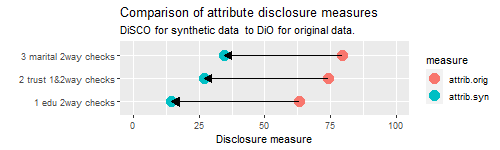
\includegraphics[width=1\linewidth]{fig2dis.png}
    \caption{Plot from \texttt{disclosure.summary} for variables flagged by checks.}
    \label{fig:f2}
\end{figure}
Returning to the example in \ref{sec:simpexamp} we now use  \texttt{disclosure.summary} for the three other variables that were not used before and 
see the plot from it in \ref{fig:f2}. All three are flagged by \texttt{check\_2way} and \texttt{trust} is also flagged by \texttt{check\_2way}. The column \texttt{check1} in the output points to the level that accounts for a high proportion of disclosures \texttt{ONE CAN`T BE TOO CAREFUL}, a response given by over 75\% of respondents. The other two variables have 2 and 9 key-target pairs, respectively, that account for many disclosures. The first of each is printed in the output. For the education variable  we see that disclosure of a school-level qualification is predicted for 17 year olds, hardly a privacy breach.
\renewcommand{\baselinestretch}{1.0}
\begin{Schunk}
\begin{Sinput}
R> disclosure.summary(s1, ods,  targets =c("edu","marital" , "trust"),
+                    keys = c("sex", "age", "region", "placesize"), 
+                    plot = FALSE, print.flag = FALSE)
\end{Sinput}
\begin{Soutput}
Disclosure risk for 5000 records in the original data

Identity disclosure measures
from keys: sex age region placesize 
For original  ( UiO )  48.38 %
For synthetic ( repU ) 14.86 %.

Table of attribute disclosure measures for the same keys, 
Original measure is  DiO and synthetic measure is DiSCO 
Variables Ordered by synthetic disclosure measure

                      attrib.orig attrib.syn                   check1 Npairs
1 edu 2way checks           63.08      14.58                               2
2 trust 1&2way checks       74.10      27.06 ONE CAN`T BE TOO CAREFUL      1
3 marital 2way checks       79.24      34.56                               9
                                                         check2
1 edu 2way checks           VOCATIONAL/GRAMMAR | 17 for key age
2 trust 1&2way checks ONE CAN`T BE TOO CAREFUL | 51 for key age
3 marital 2way checks                   SINGLE | 19 for key age
\end{Soutput}
\end{Schunk}
\renewcommand{\baselinestretch}{1.5}
The thresholds for identifying one-way and two-way relationships can be modified. In each case there are two criteria that need to be satisfied, one number and one \%. For one-way disclosure 
the parameter \texttt{thresh\_1way} has the default value of $c(50, 90)$, meaning that there must be at least 50 disclosive records for one level of a target and that $q$ values including this target must account for over 90\% of all disclosive records. For two way relationships the \texttt{thresh\_2way} has default value $c(5,80)$ and the  algorithm first identifies all 
disclosive $tq$ combinations  with denominators over 5. It then identifies the level of the key in $q$ with that best predicts this level of $t$ and checks if over 80\% of the disclosive  records with this key would have the correct prediction. 

\section{Excluding records}\label{sec:exclusions}
Having identified records where the disclosure is not really telling us anything new, one option is to  exclude some of these original records explicitly from the measures. The following parameters 
for \texttt{disclosure.summary} and \texttt{disclosure} can be used for this.
\begin{itemize}
\item{\texttt{not.target}: All records with levels of teh target given by the parameter \texttt{not.target} are excluded from all disclosure measures.}
\item{\texttt{usekeysNA}:This is set to TRUE by default so that missing values are included in all tables. It can be set to FALSE for some or all keys to exclude NAs.}
\item{\texttt{usetargetsNA)(disclosure.summary) or usetargetNA (disclosure) )}: Similar to the above for target(s) - note can be a vector for disclosure.summary.}
\item{\texttt{exclude.keys, exclude.keylevs and exclude.targetlev}For disclosure only: Three vectors of length the number of key-target pairs to be excluded from all tables.}
\end{itemize}
To illustrate exclusions we will use the Adult data set with almost 50 thousand records from the US Census income study (add refs) available as part of the \texttt{arules} package for \textbf{R} (add CRAN ref). This is one of the data sets used in \cite{giomi2022anon} to evaluate privacy risks for synthetic data. Figure \ref{fig:f3} is the output of \texttt{disclosure.summary} from the keys \texttt{age, occupation, race and sex} for the other 10 variables in the data. The code used to calculate the results in this section is in Appendix 3 \ref{sec:app3}.
The disclosiveness of the original data is relatievly low, compared to the previous example, because of the large sample size and the absence of any geographic identifiers. 
Three of the 10 variables \texttt{capital.gain, capital.loss and native.country} are flagged to check one-way relationships. The check1 column of the attribute table tells us that the levels contributing to disclosre are
zeros for the first two and \texttt{United-States} for \texttt{native.country}. These levels make up 95\%, 92\% and 89\% of all records (note maybe check what \% of disclosive).
\begin{figure}[h]
\centering
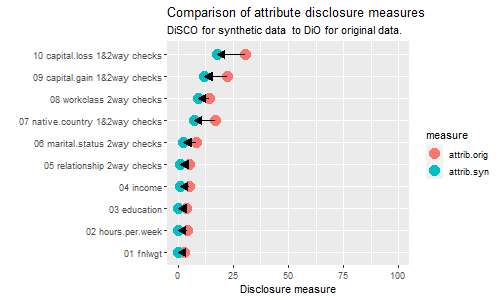
\includegraphics[width=1\linewidth]{fig3dis.png}
\caption{Plot from \texttt{disclosure.summary} for variables flagged by checks.}
\label{fig:f3}
\end{figure}
Three other variables are flagged as having disclosive two\_way relationships \texttt{workclass, marital, relationship} with totals of 7,7 and 2 $tq$ combinations respectively. The summary function \texttt{disclosure.summary} does not allow target and key specific pairs to be excluded. To
investigate this it is necessary to examine the output of \texttt{disclosure}\footnote{see code in Appendix 3 for how to do this.}. This showed that 
the largest contribution to texttt{check\_2way} for \texttt{workclass} was due to this being missing when occupation was missing, although other
relationships between these two variables also contributed. 


Table 1 gives the results of excluding different entries in the tables of $q$ and $t$ from the attrinute disclosure measures.
Excluding the levels of the target flagged by texttt{check\_1way} reduces the $DiSCO$ to almost zero for these 3 variables.
Adding exclusion of missing values reduced the disclosure for \texttt{workclass} and for some other variables a little. 
Adding the restriction to denominators of 1, reduced the disclosure for variables identified by \texttt{check\_2way} to low 
levels. In the final columns we can see that restricting to denominators of 1, by itself, gives low levels of disclosure for
all variables, with the exception of those flagged by \texttt{check\_1way}. This approach was one that was trialed in an earlier 
version of these functions but discarded for giving misleading results for some data. It can be to be too liberal in allowing some attribute disclosures that might well be found by an intruder. For example, if a record in the original data was checked and the target correctly identified
this measure would only count it if the record was unique in the original data, something that would not be known
to an intruder with no access to the original. We feel that a better approach is to exclude specific tareget/key combinations.


Adding 
\begin{table}[ht]
\centering
\begin{tabular}{|r|rr|rr|rr|rr|rr|}
  \hline
            & \multicolumn{2}{|c|} {} & \multicolumn{2}{|c|} {} & \multicolumn{2}{|c|} {} & 
      \multicolumn{2}{|c|} {denom\_lim 1} &    \multicolumn{2}{|c|} {}  \\
          & \multicolumn{2}{|c|} {} & \multicolumn{2}{|c|} {} & \multicolumn{2}{|c|} {NAs out} & 
      \multicolumn{2}{|c|} {NAs out} &    \multicolumn{2}{|c|} {}  \\
        & \multicolumn{2}{|c|} {basic} & \multicolumn{2}{|c|} {not.targetlevs} & \multicolumn{2}{|c|} {not.targetlevs} & 
      \multicolumn{2}{|c|} {not.targetlevs} &    \multicolumn{2}{|c|} {denom\_lim 1}  \\
 target & orig & syn &  orig & syn   & orig & syn  & orig & syn  & orig & syn     \\ 
  \hline
capital.gain & 22.55 & 12.09 & 0.21 & 0.00 & 0.19 & 0.00 & 0.19 & 0.00 & 2.68 & 1.12 \\ 
  capital.loss & 30.61 & 17.71 & 0.08 & 0.00 & 0.08 & 0.00 & 0.08 & 0.00 & 2.68 & 1.23 \\ 
  education & 3.71 & 0.35 & 3.71 & 0.35 & 3.43 & 0.33 & 2.45 & 0.20 & 2.68 & 0.22 \\ 
  fnlwgt & 2.70 & 0.00 & 2.70 & 0.00 & 2.47 & 0.00 & 2.45 & 0.00 & 2.68 & 0.00 \\ 
  hours.per.week & 4.36 & 0.06 & 4.36 & 0.06 & 4.06 & 0.05 & 2.45 & 0.04 & 2.68 & 0.04 \\ 
  income & 4.97 & 0.88 & 4.97 & 0.88 & 3.17 & 0.64 & 1.58 & 0.30 & 2.68 & 0.47 \\ 
  marital.status & 8.23 & 2.62 & 8.23 & 2.62 & 7.26 & 2.49 & 2.45 & 0.48 & 2.68 & 0.52 \\ 
  native.country & 17.09 & 7.28 & 0.94 & 0.02 & 0.76 & 0.02 & 0.67 & 0.01 & 2.68 & 0.71 \\ 
  relationship & 5.17 & 1.15 & 5.17 & 1.15 & 4.75 & 1.09 & 2.45 & 0.37 & 2.68 & 0.39 \\ 
  workclass & 14.27 & 9.01 & 14.27 & 9.01 & 9.14 & 3.83 & 2.45 & 0.65 & 2.68 & 0.76 \\ 
   \hline
\end{tabular}
\caption{Disclosure results from Adult data with different exclusions.}
\label{table:1}
\end{table}
\section{Conclusions}
The privacy metrics we propose here are in some sense the opposite of differential  privacy (DP).
DP claims to protect data from an intruder with arbitrary knowledge of the data, except of
the one record that has the greatest influence on the likelihood of the results. In contrast 
our metrics require the user to specify the details of what they would expect an intruder 
to know about the data. Most importantly, the user must specify keys that identify variables in the data
that would expect to be known about individuals. Also, the routines flag cases where part of the
disclosure measures come from one- or two-way relationships so that disclosure would be
expected even in the absence of data. We have evaluated the routines on a few data sets
and set levels of the thresholds for this at what seem to be reasonable levels, but 
more experience with other data sets would be valuable.

We hope that these tools will be helpful to data holders who need to make decisions 
about the risks of releasing synthetic data to the public, or to a restricted audience.
They should also enable the disclosure risks of different synthesis methods to be evaluated.


\section{Acknowledgement}
 add details...

\bibliographystyle{acm}
\bibliography{disclosure}

\section*{Appendix 1: Notation and formal definitions}{\label{sec:app1}}
Before defining the measures of identity and disclosure  risk we need to introduce the notation that will be used to calculate them. The first step is to create the quasi-identifiers from the keys for the original and synthetic data. For the keys used in the example given in Section \ref{sec:simpexamp} the  quasi-identifier that we will designate as $q$ for the first record in the original data is:

\noindent{\texttt{"FEMALE | 57 | Lubuskie | URBAN 100,000-200,000"}}

\noindent{and that for the first record in the synthetic data:}

\noindent{\texttt{"FEMALE | 39 | Zachodnio-pomorskie | URBAN 100,000-200,000"}}.

In order to calculate identity disclosure measures, we need to compare the tables of $q$ from the original and synthetic data. For attribute disclosure measures we need to cross-tabulate $q$ with each target variable $t$ and compare findings from the synthetic data with what would have been found from the original data.  In general, the levels of $q$ and sometimes $t$ in the original and synthetic data will not be the same. Before creating any tables, we need to define sets of $q$ and $t$ values that give the union of both sets of levels and align the tables so that their indices correspond.

For the original data $d_{.q}$ is the count of records with the keys corresponding to the levels of $q$ and $q_{tq}$ the count of records with this $q$ and level $t=1,...T$ of the target. The equivalent counts from the synthesised data are designated by $s_{.q}$ and  $s_{tq}$. When a member of $q$ is in the original data but not in the synthetic, $s_{.q}$ and  $s_{tq}$ are all zero. Similarly when a member of $q$ is in the synthetic data but not in the original,  $d_{.q}$ and  $d_{tq}$ are all zero. The two tables can be written as shown in Table 1, where the total records in the original data is $N_d$, made up of $N_{d~only}$ and $N_{d~both}$. The
equivalent totals  for the synthetic data are $N_s$, $N_{s~only}$ and $N_{s~both}$.

\begin{center}
\begin{table}[ht]
\begin{tabular}{ c|ccc|ccc|ccc|c} 
 &  \multicolumn{3}{|c|}{only in original} & \multicolumn{3}{|c|}{in both} & \multicolumn{3}{|c|}{only in synthetic} & Total\\
  \hline
1    & ... & $d_{1q}$  & ...   & ... & $d_{1q}$  & ...   & ... & 0 & ...  & $d_{1.}$ \\
 ... & ... & ...  & ...   & ... & ... & ...   & ... & ... & ...  & ... \\
t   & ...  & $d_{tq}$   & ...   & ... & $d_{tq}$ & ...   & ... & 0 & ...  & $d_{t.}$  \\
... & ...  & ...  & ...   & ... & ... & ...   & ... & ,,,  & ...  & ...  \\
T   & ...  & $d_{Tq}$  & ...   & ... & $d_{Tq}$ & ...   & ... & 0 &  ... & $d_{T.}$  \\
 \hline
Column sums   &  & $d_{.q}$  &   & ... & $d_{.q}$ & ...   & ... & 0 &  ... & $N_d$ \\
 \hline
Totals   &   & $N_{d\:only}$  &    &  & $N_{d~both}$ &    &  & 0 &   & $N_d$ \\
\end{tabular}
\end{table}
\begin{table}[ht]
\begin{tabular}{ c|ccc|ccc|ccc|c} 
 &  \multicolumn{3}{|c|}{only in original} & \multicolumn{3}{|c|}{in both} & \multicolumn{3}{|c|}{only in synthetic} & Total\\
  \hline
1    & ... & 0  & ...   & ... & $s_1q$ & ...   & ... &  $s_1q$ & ...  & $s_{1.}$ \\
 ... & ... & ...  & ...   & ... & ... & ...   & ... & ... & ...  & ... \\
t   & ...  & 0  & ...   & ... & $s_tq$  & ...   & ... &  $s_tq$ & ...  & $s_{t.}$ \\
... & ...  & ...  & ...   & ... & ... & ...   & ... & ... & ...  & ...  \\
T   & ...  & 0  & ...   & ... & $s_Tq$  & ...   & ... & $s_Tq$ &  ... & $s_{T.}$ \\
 \hline
Column sums   & ...  & 0  & ...   & ... & $s_{.q}$ & ...   & ... & $s_{.q}$ &  ... & $N_s$ \\
 \hline
Totals   &   & 0  &    &  & $N_{s~both}$ &    &   &   & $N_{s\:only}$ & $N_s$ \\

\end{tabular}
\caption{Notation for tables from quasi-identifier ($q$) and target ($t$) from original (upper table) and synthetic data (lower table).}
\end{table}
\end{center}
To calculate the \% of records in the original and synthetic data we need:
\begin{equation}
    \%~Unique~in~Original = UiO = 100\sum{(d_{.q} |d_{.q} = 1})/N_d. 
\end{equation}
\begin{equation}
    \%~Unique~in~Synthetic = UiS = 100\sum{(s_{.q} |d_{.q} = 1})/N_d.
\end{equation}
The intruder has information about the keys for an individual in the real data that they attempt to identify in the synthetic data. If they find a  unique record in the synthetic data, they might claim to have identified them. This leads to one possible identity disclosure measure for synthetic data as:
\begin{equation}
    \%~Unique~in~Synthetic~in~Original = UiSiO = 100 \sum{(d_{.q} = 1 |s_{.q} = 1 \land d_{.q} > 0})/N_d.
\end{equation}
This measure would include records that are not unique in the original data, so a further identity disclosure measure requires the combination of keys to be unique in both data sets, giving:
\begin{equation}
    \%~replicated~Uniques = repU = 100\sum{(s_{.q} |d_{.q} = 1 \land s_{.q} = 1)}/N_d.
\end{equation}

To find an attribute from a set of keys, it is necessary to examine the distribution of $s_{tq}$ for groups defined by $q$. We define column proportions for the original and synthetic data as $pd_{tq} = d_{tq}/d_{.q}$ and for the synthetic as $ps_{tq} = s_{tq}/s_{.q}$.

Returning to the scenario described in Section \ref{subsec:scen}, we must first define a measure of attribute disclosure for the original data. This is based on the concept of \textit{l-diversity} \cite{ldiv} that requires that each set of records defined by $q$ has at least $l(\ge{2}$ distinct values of the target. A data set is \textit{l2-diverse} for $q$ and $t$ if all records for every $q$ have the same level of $t$\footnote{This could be generalised to $l>2$, but in practice the levels of targets are not generally exchangeable and a more practical approach would be to aggregate levels for certain targets.} An attribute disclosure measure for the original data can be defined as \textit{\% Disclosive in Original} :
\begin{equation}
  DiO = 100\sum{(d_{tq} |pd_{tq} = 1})/N_d.
\end{equation}

An intruder with access only to the synthetic data, but with knowledge  of $q$ from one or more individuals in the original, would look them up in the synthetic data. Some of their $q$ levels be key combinations that do not appear in the synthetic data
leaving the proportion that do appear as $KiOiS$ (Keys in original in Synthetic) 
\begin{equation}
  KiSiO = 100\sum{(d_{.q} |ps_{tq} = 1})/N_d.
\end{equation}
For those that are found some will identify a level of $t$ that does not occur for 
this $q$ in the original data, excluding these gives the measure $DiSiO$ (Disclosive in Synthetic in Original). But this measure might point to some records where $q$ in the original may not give a unique level of $t$. By requiring the disclosure to point to records where $q$ gives the unique correct target in the original we get $DiSCO$ (Disclosive in Synthetic Correct in Original), our preferred disclosure measure:
\begin{equation}
 DiSCO = 100\sum{(d_{tq} |ps_{tq} = 1 \land pd_{tq} = 1 \land s_{tq} = d_{tq}})/N_d.
\end{equation}

Note that $DiSCO$ can include records that are not unique in the synthetic data. This restriction can be imposed by requiring the denominator in the synthetic data to exceed a given limit, as described in Section \ref{sec:exclusions}.

\section*{Appendix 2: CAP measures }{\label{sec:app2}}
The following measures are calculated by the function \texttt{disclosure} and are stored in the component \texttt{allCAPs} of the output object of class \texttt{disclosure} that is printed when the parameter \texttt{to.print} includes \texttt{allCAPs}. Each measure is an average of the Correct Attribution Probability (CAP) averaged for different situations. The first measure is known as the baseline CAP and refers to an average of the predictions that would be made by someone who only has access to the marginal distribution of the target. The intruder then guesses the CAP for each level of the target according to the relative frequencies $pd_{t.}$. Averaging this over all observations gives
\begin{equation}
   \nonumber  baseCAPd = 100\sum{(pd_{t.})^2}/N_d.
\end{equation}
The next two measures are the CAP that would be obtained for someone with access to only the original data or only the synthetic data and in each case predicting $t$ from $q$. This gives
\begin{equation}
   \nonumber  CAPd = 100\sum\limits_q{(pd_{.q})}(\sum\limits_t{pd_{tq}^2)})
\end{equation}
for the original data and the equivalent measure for the synthetic data as $CAPs$. 
For DCAP we need the probability of a prediction made from the synthetic data being correct in the original giving:
\begin{equation}
   \nonumber  DCAP = 100\sum\limits_{tq}{(ps_{tq}}d_{tq})/N_d
\end{equation}

 and
\begin{equation}
   \nonumber  TCAP = 100\sum\limits_{tq}{(ps_{tq}}d_{tq} | pd_{tq} = 1)/N_d.
\end{equation}
The DCAP and TCAP measures can be compared with CAPd. Some authors \cite{little2022,lotte} have suggested subtracting baseCAPd from DCAP to adjust for the baseline AP of the target, although this may sometimes lead to negative estimates.
\begin{Schunk}
\begin{Sinput}
R> print(t5, to.print = "allCAPs")
\end{Sinput}
\begin{Soutput}
Disclosure measures from synthesis for 5000 records in original data
CAP measures for the target depress with keys
sex age region placesize 

  baseCAPd  CAPd  CAPs  DCAP TCAP
1     9.81 74.15 69.78 16.39 5.98
2     9.81 74.15 69.66 16.30 5.51
3     9.81 74.15 69.10 15.88 5.23
4     9.81 74.15 68.83 15.87 5.07
5     9.81 74.15 68.88 17.30 5.89
\end{Soutput}
\end{Schunk}
\section*{Appendix 3: Code for analysis of teh Adult data set as described in \ref{sec:}}{\label{sec:app3}}
\renewcommand{\baselinestretch}{1.0}
\begin{verbatim}
library(arules)
data(AdultUCI)
##syn.AdultUCI <- syn(AdultUCI....) gives warning about "-" in variable names
names(AdultUCI) <- gsub("-",".", names(AdultUCI))
dim(AdultUCI)
names(AdultUCI)
##------ drop one of two identical education variables---------------------------
adultsample <- AdultUCI[,-c(5)]
##------ native.country moved to end as many levels that slow down synthesis-----
synadult <- syn(adultsample, visit.sequence = c(1:12,14,13) ,seed = 7868) 
##------ get basic disclosure and make Figure 3----------------------------------
dd1 <- disclosure.summary(synadult,adultsample,
            keys = c("age" , "occupation","race", "sex" ))
png("vignettes/fig3dis.png",height=300, width=500)
print(dd1)
dev.off()
##------ exclude some target levels and missing values for targets---------------
dd2 <- disclosure.summary(synadult,adultsample, print.flag = FALSE,denom_lim =1, 
                   exclude_ov_denom_lim  = TRUE, 
                   keys = c("age" , "occupation","race", "sex" ))
##------ exclude some target levels and missing values for targets---------------
dd3 <- disclosure.summary(synadult,adultsample, print.flag = FALSE,denom_lim =1, 
                   not.targetslev = c(rep("",5),"0","0","United-States"),
                   keys = c("age" , "occupation","race", "sex" ))
                   dd1 <- disclosure.summary(synadult,adultsample,  keys = c("age" , "occupation","race", "sex" ))
##-------restrict to denominators of 1 -----------------------------------------
dd4 <- disclosure.summary(synadult,adultsample, denom_lim =1, 
                          not.targetslev = c(rep("",5),"0","0","","United-States",""),
                          usekeysNA = FALSE, usetargetsNA = FALSE, 
                          exclude_ov_denom_lim  = TRUE, 
                          keys = c("age" , "occupation","race", "sex" ))
##----------just denominators not others---------------------------------------
dd5 <- disclosure.summary(synadult,adultsample, denom_lim =1, 
                          exclude_ov_denom_lim  = TRUE, 
                          keys = c("age" , "occupation","race", "sex" ))
##-----------make table 1------------------------------------------------------
library(stringr)
cols12 <- dd1$attrib.table[,1:2]
   dimnames(cols12)[[1]] <- word(dimnames(cols12)[[1]],2,2)
cols34 <- dd2$attrib.table[,1:2]
   dimnames(cols34)[[1]] <- word(dimnames(cols34)[[1]],2,2)
cols56 <- dd3$attrib.table[,1:2]
   dimnames(cols56)[[1]] <- word(dimnames(cols56)[[1]],2,2)
cols78 <- dd4$attrib.table[,1:2]
   dimnames(cols78)[[1]] <- word(dimnames(cols78)[[1]],2,2)
cols910 <- dd5$attrib.table[,1:2]
    dimnames(cols910)[[1]] <- word(dimnames(cols910)[[1]],2,2)
table.adult <- data.frame(cols12[order(dimnames(cols12)[[1]]),],
                          cols34[order(dimnames(cols34)[[1]]),],
                          cols56[order(dimnames(cols56)[[1]]),],
                          cols78[order(dimnames(cols78)[[1]]),],
                          cols910[order(dimnames(cols910)[[1]]),])
##--------------------- check 2way for one target------------------------------
dis1 <- disclosure(synadult,adultsample, target = "workclass",
                   keys = c("age" , "occupation","race", "sex" ))
print(dis1, to.print = c("attrib","check\_2way"))
\end{verbatim}
\renewcommand{\baselinestretch}{1.5}
\end{document}
